\documentclass[12pt,a4paper]{article}
\usepackage{german}
\usepackage[utf8]{inputenc}
\usepackage[T1]{fontenc}
\usepackage{ae}
\usepackage{amssymb}
\usepackage{ifthen}
\ifx\pdfoutput\undefined
\usepackage[dvips]{graphicx}
\else
\usepackage[pdftex]{graphicx}
\pdfcompresslevel=9
\pdfpageheight=297mm
\pdfpagewidth=210mm
\usepackage{color}
\usepackage{hyperref}

\definecolor{uniblue}{rgb}{0, 0.2, 0.4}

\newcommand{\cmark}[1]{{\color{uniblue} \textbf{#1}}}


\hypersetup{
colorlinks=true,
pdfpagemode=UseNone,
pdfstartview=FitH,
pdfview=FitH,
urlcolor=uniblue,
linkcolor=uniblue
}
\fi
%%
\errorcontextlines=999
%
%
\def\hs#1{\hspace*{#1cm}}
\def\spiegel#1{$\stackrel{\leftarrow}{#1}$}
\def\mspiegel#1{\stackrel{\leftarrow}{#1}}
\def\ei#1{$\ \stackrel{(#1)}{=}\ $}
\def\mei#1{\ \stackrel{(#1)}{=}\ }
\def\als{~~~$\simeq$~~~}
\def\ab{$\stackrel{uses}{\longrightarrow}\ $}
%
%
\setlength{\textwidth}{175mm}
\setlength{\oddsidemargin}{0mm}
\setlength{\evensidemargin}{0mm}
\setlength{\topmargin}{0mm}
\setlength{\textheight}{252mm}
\setlength{\voffset}{-2.4cm}
\setlength{\hoffset}{-1.2cm}
\parskip1ex
\parindent0cm
%%
\def\rand#1{\marginpar{\tiny #1}}
\def\co#1{$\overline{\mbox{#1}}$}
\def\mco#1{\overline{\mbox{#1}}}         
\def\rhd{\vartriangleright}
\def\mouver{\vartriangleright\ }
\def\ouver{$\vartriangleright\ $}
\def\folgt{$\ \Longrightarrow\ $}
\def\gdw{$\ \Longleftrightarrow\ $}
\def\rhd{$\vartriangleright$}
\def\lhd{$\vartriangleleft$}
\def\brhd{$\blacktriangleright$}
\def\blhd{$\blacktriangleleft$}
\def\bst{$\bigstar$}
\def\ost{$\circledast$}
%%%
\def\err#1{$error_{#1}$}
\def\merr#1{error_{#1}}
%
\def\tsig{$T_{SIG}$}
%
\def\mt{$\times\ $}
\def\pot#1{{\Large $\wp$}(#1)}
\def\mpotf#1{{\Large \wp_{fin}}(#1)}
\def\ab{$\stackrel{uses}{\longrightarrow}\ $}
\def\wird{~{\tt ==>}~}
\def\move{~\vdash~}
\def\mv#1{~\stackrel{#1}{\vdash}~}
\def\moves{~\stackrel{*}{\vdash}~}
\def\movep{~\stackrel{+}{\vdash}~}
\def\regel{\ \longrightarrow\ }
\def\wirdm{\ \Longrightarrow\ }
\def\wirds{~\stackrel{*}{\Longrightarrow}~}
\def\alt{\ \vert\ }
%
%
\def\ww{{\tt \#t$\ $}}
\def\ff{{\tt \#f$\ $}}
\def\mww{\mbox{\tt \#t}}
\def\mff{\mbox{\tt \#f}}
%
\def\bool{I\hskip -1.6pt B$\ $}
\def\mbool{\rm I\hskip -1.6pt B}
%
\def\pot#1{{\Large $\wp$}(#1)}
\def\mrea{\rm I\hskip -1.6pt R}
\def\mnat{\rm I\hskip -1.6pt N}
\def\mnato{\rm I\hskip -1.6pt N_0}
\def\rea{I\hskip -1.6pt R$\ $}
\def\nat{I\hskip -1.6pt N$\ $}
\def\nato{I\hskip -1.6pt N_0$\ $}
\def\aus{$ \in\ $}
\def\bull{\vrule height .9ex width .8ex depth -.1ex }
\def\gdw{:$\Longleftrightarrow$}
\def\folgt{$\ \Longrightarrow\ $}
%
\def\se{$\ \bullet\ \ $}
\def\pa{$\ \parallel\ \ $}
\def\async{$\ \equiv\hskip -6pt\equiv\hskip -3pt\gg\ \ $}
\def\sync{$\ \bowtie\hskip -6pt\rhd\ \ $}
\def\nix{$\ \infty\ $}
\def\ka{$\cal K$}
\def\seperate{\hrule\vskip 2pt\hrule\vskip 2pt\hrule}
%
\def\seperate{\hrule\vskip 2pt\hrule\vskip 2pt\hrule}
%
\newcounter{beispiel}
\newenvironment{bsp}[2]{\label{#1}\addtocounter{beispiel}{1} \vskip 8pt
\seperate \vskip 6pt
{\bf Beispiel \thechapter.\thebeispiel:} ({\em #2}) \vskip -3pt }
{\vskip 6pt
\seperate \vskip 5pt}
%
\def\strich{\begin{center} \rule{7cm}{2pt} \end{center}}
%
\newenvironment{remark}{\begin{description}\item {\bf Bemerkung:} }
{ \end{description}}
%
% ***************************************************************
\def\eg#1{eg(#1)}
\def\ag#1{ag(#1)}
\def\bs{\vskip 0.7cm}
%
%
\newcommand{\bildw}[4]{
  \begin{figure}[htb]
    \begin{center}
      \includegraphics[width=#4 cm]{images/#2}
      \caption{#3}
      \label{#1}
    \end{center}
  \end{figure}
}
%
%
\newcommand{\bildh}[4]{
  \begin{figure}[hbt]
    \begin{center}
      \includegraphics[height=#4 cm]{images/#2}
      \caption{#3}
      \label{#1}
    \end{center}    
  \end{figure}
}
%
%
\newcommand{\bild}[3]{
  \begin{figure}[hbt]
    \begin{center}
      \includegraphics[width=\textwidth]{#2}
      \caption{#3}
      \label{#1}
    \end{center}    
 \end{figure}
}
%
%
\newcommand{\atitle}{
  \begin{center}
    \begin{minipage}[t]{16cm}
      \begin{minipage}{3cm}
        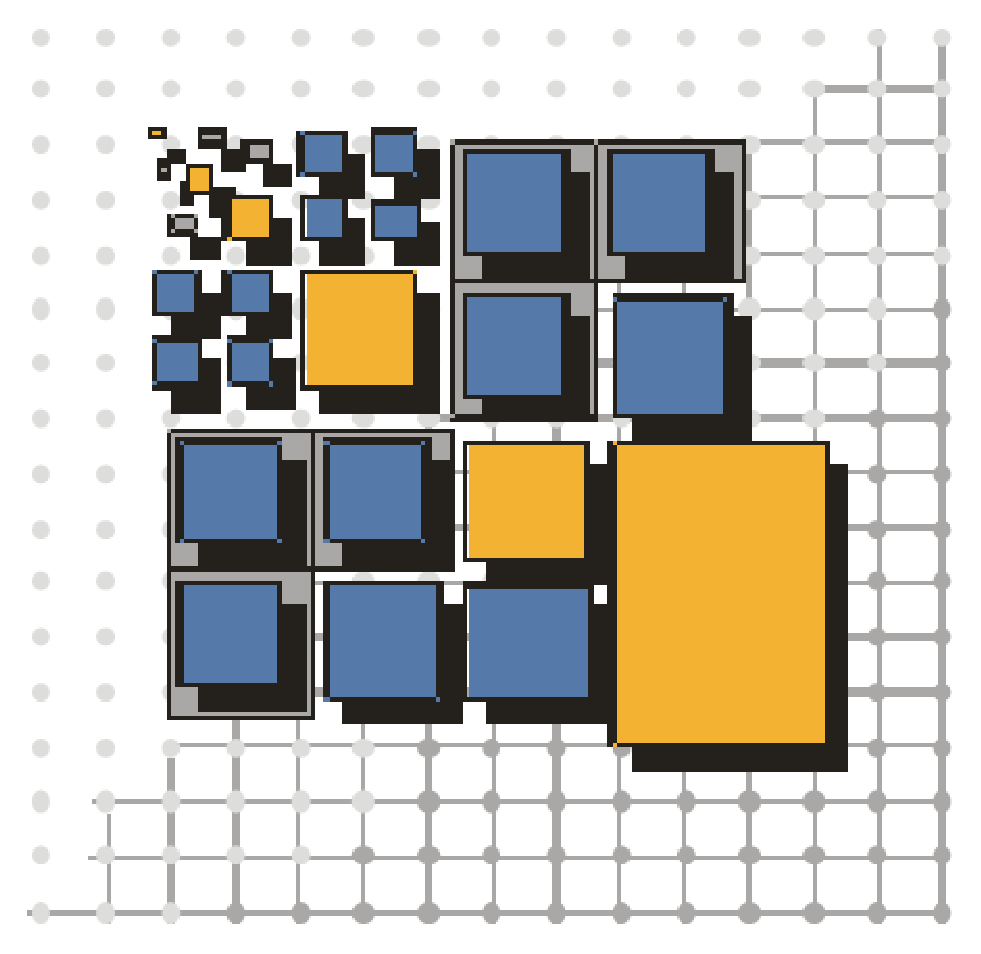
\includegraphics[height=26mm]{images/vs-logo}
      \end{minipage}
      \hfill
      \begin{minipage}{9cm}
        \centering
        {\small University of Bamberg\\}
        {\Large Distributed Systems Group\\}
			 \vspace{0.3cm}
      \end{minipage}
      \hfill
      \begin{minipage}{3cm}
        
\includegraphics[height=26mm]{images/uni}
      \end{minipage}
    \end{minipage}\\[7ex]
  \end{center}
  \ifx\pdfoutput\undefined
  \else
  \hypersetup{
    pdfauthor={Distributed Systems Group},
    pdfsubject={Richtlinien zur Erstellung von Seminar- und Abschlussarbeiten},
    pdftitle={Richtlinien zur Erstellung von Seminar- und Abschlussarbeiten}
  }
  \fi
}
%
%
\newcommand{\cci}{\\[-6ex]}
\newcommand{\cc}{\\[-4.5ex]}
%
%
\newcounter{LAufgabe}
\newenvironment{LAufgabe}{
  \addtocounter{LAufgabe}{
    \large\sc L\"osungsvorschlag  zu Aufgabe
    \theLAufgabe\\[1ex]
  }
}
{\vspace{0.5ex}}
%
%
\newcounter{Aufgabe}
\newenvironment{Aufgabe}{
  \addtocounter{Aufgabe}{1}{
%    \large\sc Aufgabe \theAufgabe\\[1ex]
  }
}
{\vspace{0.5ex}}
%
%
\newcommand{\No}{\N_0}
\newcommand{\N}{\mathbb{N}}
\newcommand{\R}{\mathbb{R}}
\newcommand{\Z}{\mathbb{Z}}
\newcommand{\Q}{\mathbb{Q}}
%
\newcommand{\Ltitel}[1]{
{~\\[-2.5cm] 
\begin{center}
\Large\sc Informatik I~$\cdot$~
{\LARGE\sc \"Ubungsblatt #1}~$\cdot$~WiSe 1997/98
\end{center}~\\[-52pt]}{\LARGE\sc
~\begin{center}
L\"osungsvorschl\"age\\[4ex]
\end{center}
}}
%
%
\newcommand{\link}[2]{
  \ifx\pdfoutput\undefined
  #1 (#2)
  \else
  \href{#2}{#1}
  \fi  
}

%%% Local Variables: 
%%% mode: latex
%%% TeX-master: "ueb1"
%%% TeX-master: t
%%% TeX-master: t
%%% End: 

%
\begin{document}
% Vorlesung, Blatt-#, Autor, Key-Words (mit Kommata)
\atitle
%
\begin{center}
{\bf\huge Richtlinien zur Erstellung von Seminar-, Bachelor- und Masterarbeiten}

{\it Stand: April 2019}
\end{center}
%
\section{Aufbau von Bachelor-, Master- und Seminararbeiten}
%
Zur Erstellung von Seminar-- und Abschlussarbeiten sind die vom Lehrstuhl im allgemeinen DSG--Kurs\footnote{\url{https://vc.uni-bamberg.de/moodle/course/view.php?id=2139}} bereitgestellten Vorlagen zu verwenden, da in diesen das Titelblatt, die verschiedenen Verzeichnisse und Formatierungen bereits definiert sind.

\subsection{Verzeichnisse}

Am Anfang der Arbeit direkt nach der Titelseite befinden sich folgende Verzeichnisse:

\begin{itemize}
	\item Inhalts-,
	\item Abbildungs-,
	\item Tabellen-,
	\item Listings-
	\item und Abkürzungsverzeichnis.
\end{itemize}
	
Die Inhalts-, Abbildungs-, Listings- und Tabellenverzeichnisse werden in allen Vorlagen automatisch
erstellt, wenn die dazu vorgesehenen Formatierungsvorschriften für Bilder und Tabellen
und deren Beschriftungen eingehalten werden\footnote{Siehe Dokumentationen zu Word bzw. LaTeX oder vom Lehrstuhl bereitgestelltes HowTo.}. 
Das Abkürzungsverzeichnis nimmt alle
in der Arbeit verwendeten Abkürzungen in alphabetischer Reihenfolge auf, jedoch keine
darüber hinausgehenden Abkürzungen. Ausgeschlossen hiervon sind allgemein bekannte
Abkürzungen wie 'ff.', 'z.B.' oder 'o.'. Abkürzungen sind bei ihrer ersten Verwendung
auszuschreiben und die Abkürzung hinter dem ausgeschriebenen Wort in Klammern anzugeben.

\textit{Beispiel}: Im Text -- "`...hierzu wurde das \textit{Java Development Kit} (JDK) in der Version..."'\\
Eintrag im Abkürzungsverzeichnis -- "`\textit{JDK} \hspace{10pt} Java Development Kit"'.


Nicht benötigte Verzeichnisse sind vor Abgabe der Arbeit aus dieser zu entfernen. Nach
den Verzeichnissen schließt sich der Hauptteil der Arbeit an.

\subsection{Hauptteil}
Nach den Verzeichnissen beginnt mit dem Hauptteil die eigentliche Ausarbeitung. 
Den Aufbau des Hauptteils sollten Sie grundsätzlich mit Ihrem Betreuer abstimmen. Als Anhaltspunkt für eine Gliederung kann folgender Aufbau dienen:\\
Der Hauptteil der Arbeit beginnt mit einer Einleitung, die das Thema der Arbeit erläutert
und es hinreichend motiviert. Nach der Einführung und Motivation wird ein kurzer
Überblick über das Vorgehen und die Kapitel der Arbeit gegeben, um dem Leser ein 'big
picture' zu vermitteln. Die Arbeit wird durch eine Zusammenfassung beendet, in der zentrale Ergebnisse kurz geb\"undelt und die gesamte Arbeit bewertet
wird\footnote{Bspw. Gegenüberstellung von Vor- und Nachteilen verwendeter Methoden, selbst entwickelter Lösungen,
etc.}. Darüber hinaus sollte die Zusammenfassung einen Ausblick auf weitere Entwicklungsmöglichkeiten des in der Arbeit behandelten Themas geben.

\subsection{Zitate und Literaturverzeichnis}

Die Arbeit beruht auf \textit{gründlich} recherchierten
Literaturquellen, die in geeigneter Weise in der Arbeit referenziert werden müssen.
Ins Literaturverzeichnis werden die folgenden Arten von Quellen aufgenommen:
\begin{itemize}
	\item (Lehr-)Bücher,
	\item Artikel in wissenschaftlichen Journalen,
	\item Beiträge zu Konferenzen und Workshops,
	\item Wissenschaftliche Arbeitsberichte ("`TechReports"')
	\item und Standards
\end{itemize}

Quellen sollten so ausführlich im Literaturverzeichnis beschrieben werden, dass sie eindeutig identifizierbar und wieder auffindbar sind. 
Grundsätzlich immer anzugeben sind Autor und Titel, weitere Mindestangaben sind abhängig vom konkreten Typ der Quelle: 

\begin{itemize}
	\item Bücher: Autor, Titel, Auflage, Verlag, Datum\footnote{mind. Jahr, nach Möglichkeit sollte auch der Monat mit angegeben werden}
	\item Beiträge in Journalen: Autor, Titel, Journalname (+Kürzel des Journals), Volume, Number, Seitenzahlen
	\item Beiträge zu Konferenzen und Workshops: Autor, Titel, Konferenzname (+Kürzel der Konferenz), Ort, Datum, Seitenzahlen
	\item Arbeitsberichte: Autor, organisationale Zugehörigkeit (bspw. Universität), Titel, Datum
	\item Standards: Name der ausgebenden Organisation (einzelne Autoren sollen nicht aufgeführt werden), Titel, Version, Datum
\end{itemize}

Nicht ins Literaturverzeichnis aufgenommen werden, alle nichtwissenschaftlichen Quellen\footnote{insb. Webseiten, Handbücher, Artikel aus nicht-wissenschafltichen Zeitschriften (z.B. \textit{c't}), etc.}. Bei Zitaten aus diesen Quellen, muss stattdessen eine Fußnote genutzt werden. 
Grundsätzlich als Quelle ausgeschlossen sind alle zu einem gleichen
Zweck (Abschlussarbeit, Hausarbeit) oder zum Zweck der Lehre (außer Lehrbüchern)
erstellten Dokumente. 
Bei strittigen Fällen ist der Betreuer der Arbeit zu fragen, ob eine Quelle ins Literaturverzeichnis aufgenommen werden soll oder ob sie generell unzulässig ist.

Auf verwendete Quellen kann durch ein direktes oder indirektes Zitat Bezug genommen
werden. Diese sind entsprechend zu kennzeichnen. Ein direktes Zitat liegt bei einer wörtlichen
Übernahme aus einer Quelle vor. Ein Zitat ist indirekt, wenn in Anlehnung an
die Gedanken eines Autors ein Sachverhalt mit eigenen Worten dargestellt wird oder die
Gedanken eines Autors mit eigenen Worten nachvollzogen werden.

Direkte Zitate sind durch Anführungszeichen von anderem Text zu unterscheiden und die
Quelle des Zitates ist im Text mit der Nummer der Quelle aus dem Literaturverzeichnis
und mit Seitenangabe zu referenzieren. Beispiel: "`Dies ist ein wörtliches Zitat aus einer
Quelle"' ([22] S. 231 f.). Werden im direkten Zitat Satzteile weggelassen ist dies durch
'[...]' zu kennzeichnen. Zum besseren Verständnis hinzugefügte Satzteile sind ebenfalls
in eckige Klammern einzuschließen. Weitere Änderungen am Text (bspw. unterstreichen,
hervorheben) sind ggf. durch eine Bemerkung als eigene Änderungen kenntlich zu machen.
Wird wortwörtlich aus einer anderen Sprache übersetzt ist die verwendete Passage wie
ein direktes Zitat zu behandeln und mit einem Vermerk zu versehen, dass es sich um eine
Übersetzung aus der jeweiligen Sprache handelt. Indirekte Zitate sind ebenfalls im Text
mit der Nummer aus dem Literaturverzeichnis und einer Seitenangabe zu referenzieren.
Im Gegensatz zum direkten Zitat wird aber hier ein 'vgl.' vorangestellt. Dabei sind Zitate
über zwei Seiten mit f. (folgende) nach der Seitenzahl, Zitate über drei bis fünf Seiten
kennzeichnen mit ff. (fortfolgende) und Zitate über mehr als fünf Seiten mit genauer
Seitenangabe (Bsp.: S. 15--23) zu versehen.

\subsection{Anhang}

Nach dem Literaturverzeichnis kann sich bei Bedarf ein Anhang anschließen, in den weitere
Erläuterungen, Abbildungen, Tabellen etc. aufgenommen werden können, die das
Verständnis der Arbeit verbessern, aber nicht zentral für deren Verständnis sind. Dies
ist besonders relevant für Bachelor- und Masterarbeiten, bei denen im Anhang bspw. wichtige Teile
des Sourcecode\footnote{Eine Darstellung des gesamten Sourcecodes ist nicht erwünscht.}, 
der im Hauptteil der Arbeit nur auszugsweise abgebildet wurde, oder
vollständige UML--Diagramme gezeigt werden können, die vorher nur auszugsweise in der
Arbeit verwendet wurden. 

Die letzte Seite einer Abschlussarbeit muss die vom Prüfungsamt geforderte Eigenständigkeitserklärung enthalten.

\newpage
\section{Abgabe}

Die Abgabe von Abschlussarbeiten erfolgt nach den in der Prüfungsordnung festgelegten Regeln. 
Bei Abschlussarbeiten mit einem praktischen Teil wird der Sourcecode,
ggf. UML-Modelle, benötigte Bibliotheken etc. sowie die kompilierte Software auf einer CD
der Arbeit beigelegt. Zusätzlich zur Abgabe der Abschlussarbeit beim Prüfungsamt,
ist die Arbeit im PDF--Format beim Betreuer (z.B. per E-Mail o. auf der beigelegten
CD) abzugeben.

Die Abgabe von Seminararbeiten ist mit dem jeweiligen Betreuer zu klären. In
der Regel werden Seminararbeiten am Tag der Abgabe im PDF--Format per Email beim
Betreuer abgegeben. 

\section{Bewertung von Seminar- und Abschlussarbeiten}

Die Bewertung der Arbeiten erfolgt sowohl nach inhaltlichen als auch formalen Kriterien,
weshalb es erforderlich ist, die hier beschriebene Form der Arbeit einzuhalten.
Es ist auch darauf zu achten, dass die Arbeit keine großen sprachlichen Mängel
(Rechtschreib-, Grammatikfehler) aufweist. Insbesondere ist auch auf die korrekte Angabe
und Referenzierung von verwendeten Quellen zu achten, da bei inkorrekter Zitierung
die Arbeit als nicht ausreichend bewertet werden kann.


\section{Anmerkungen zu Microsoft Word und \LaTeX}


Im allgemeinen VC-Kurs stellt der Lehrstuhl Vorlagen sowohl für LaTeX als auch Microsoft Word zur Verfügung. Für beide Vorlagen gilt, dass an den voreingestellten Abständen und Formatierungen
nichts verändert werden darf. 
\textbf{Der Lehrstuhl empfiehlt generell die Verwendung der TeX/LaTeX--Vorlage, }
da hier besonders die Erstellung und Verwaltung des Literaturverzeichnisses
automatisch mit Hilfe von BibTeX vorgenommen wird.

Hilfreiche Informationen zur Nutzung von LaTeX finden Sie in unserer Vorlage "`dsg-seminar-mit-anleitung"'.
%
\end{document}